% !TeX root = report.tex

\documentclass[12pt]{article}
\usepackage{lingmacros}
\usepackage{tree-dvips}
\usepackage[utf8]{inputenc}
\usepackage{fancyhdr}
\usepackage{listings}
\usepackage{subfig}
\usepackage{floatrow}
\usepackage{float}
\usepackage{xcolor}
\usepackage{geometry}
\usepackage{graphicx}
\usepackage{wrapfig}
\usepackage{amsmath}
\usepackage{hyperref}

%% papir layout
\geometry{
a4paper,
total={170mm,257mm},
left=15mm,
top=20mm,
}

%% Layout og farve til hyperlinks
\definecolor{link}{rgb}{0,0,215}
\hypersetup{
    colorlinks=true,
    linkcolor=link,
    filecolor=link,      
    urlcolor=link,
    citecolor=link,
    pdfpagemode=FullScreen,
}

\graphicspath{ {./img} } %% path to images

%% Litteraturliste
\usepackage{biblatex}
\addbibresource{litteratur.bib}

%% Code style
\definecolor{comment}{rgb}{0,0.45,0}
\definecolor{codegray}{rgb}{0.5,0.5,0.5}
\definecolor{codepurple}{rgb}{0.58,0,0.82}
\definecolor{backcolour}{rgb}{0.95,0.95,0.92}
\lstdefinestyle{CodeStyle}{
    backgroundcolor=\color{backcolour},   
    commentstyle=\color{comment},
    keywordstyle=\color{magenta},
    numberstyle=\tiny\color{codegray},
    stringstyle=\color{codepurple},
    basicstyle=\ttfamily\footnotesize,
    breakatwhitespace=false,         
    breaklines=true,                 
    captionpos=b,                    
    keepspaces=true,                 
    numbers=left,                    
    numbersep=5pt,                  
    showspaces=false,                
    showstringspaces=false,
    showtabs=false,                  
    tabsize=2
}
\lstset{style=CodeStyle}
\lstdefinelanguage{JavaScript}{
  keywords={typeof, new, true, false, catch, function, return, null, catch, switch, var, if, in, while, do, else, case, break},
  keywordstyle=\color{purple}\bfseries,
  ndkeywords={class, export, const, var, let, boolean, throw, implements, import, this, !!, !=, ===, ;},
  ndkeywordstyle=\color{blue}\bfseries,
  identifierstyle=\color{black},
  sensitive=false,
  comment=[l]{//},
  morecomment=[s]{/*}{*/},
  commentstyle=\color{comment}\ttfamily,
  stringstyle=\color{orange}\ttfamily,
  morestring=[b]',
  morestring=[b]"
}

%%%%%%% Document begin %%%%%%%%%%%
\begin{document}

\title{kompression}
\author{Johannes Jørgensen\\ S2o}
\date{Maj 2022}
\maketitle
\pagebreak
\tableofcontents
\pagebreak

%% Introdoktion
\section{introduktion}
Denne PDF-fil du læser i, har en filstørrelse på omkring 1.2 KB. 
Et gennemsnitligt billede med billedformaten JPG har en størrelse på 11.8 KB,\cite*{Solarwinds/filesizes} og en time lang Fuld HD-video har en størrelse på 1.2 GB.\cite*{filecatalyst/movesizes} 
Det er mindre effektivt, dyre og langsommere at sende større filer verden rundt via internettet. Men det er her kompression kommer ind i billedet. 
Kompression er en måde at reducere data, at indkode færre bits end den originale repræsentation af givende data. Hver kompression af et stykke data kan enten være ”Lossy” eller ”Lossless”.\cite*{Wiki/dataCompression} 
Lossless kompression er en reduktion af data uden noget data går tabt, hvor lossy kompression er hvor noget af den originale data bliver slette.
\section{LZ77 Algoritme}

LZ77 (også kaldt LZ1) algoritme er en lossless data kompression algoritme udviklet af Lempel og Ziv i 1977. 
Der er flere forskellige variationer af LZ77 algoritmen (LZ78 samt LZSS) og algoritmerne kan bruges til forskellige formål. Men alle af LZ-algoritmerne grundlæggende princip er det samme. 
Algoritme-serien er adopteret af mange forskellige systemer, mest kendt i GIF og DEFLATE algoritmen som bruges i ZIP og PNG.\cite*{Wiki/LZ77}\\\newline
Den grundlæggende algoritme LZ77 komprimerer gentagende data med at referater, som tidligere eksisterede data i den ukomprimerede data. Referatet til det gentaget data bliver til et talpar, 
dette kan også kaldes for en ”pointer”. Udsagnet ”pointer” er et tal (en integrer) som refererer til et stykke data’s adresse i hukommelsen. 
Talparet er kaldt ”length-distance pair”, som svare til udsagte ”hvert af de næste længdetegn er lig med tegnene nøjagtigt afstandstegn bagved i den ukomprimerede strøm”. 
Talparet er et output af tal (\boldmath(D)istance, \boldmath(L)ength, \boldmath(c)harater) som er defineret ved:
\[[D,L,c]\] 
\begin{itemize}
  \item \boldmath(D): Afstanden for antal positioner, der flyttes bagud for at finde starten af den matchende data.
  \item \boldmath(L): Længden af det matchende data.
  \item \boldmath(c): Karakteren som er repræsenteret efter det matchende data er fundet.
\end{itemize}
LZ77 algoritmen itererer (køre igennem/gentag) igennem et stykke data, for at finde den længste sekvens af data som bliver brugt flere gange. Sker der et match i et par datastykker, 
bliver de matchene datastykker gemt.

\subsection{Eksempel og gennemgang}
En måde at kunne visualisere LZ77 algoritmen er med en gennemgang af et eksempel. For at kunne simplificere hvad algoritmen gør, bruger jeg en streng med gentagende bogstaver. 
LZ77 er ikke kun brugbar i tekst kompression, men også andre dataformater.\cite{yt/LZ77}\\
Eksempel streng er til kompression:\\
\[AABCBBABC\]
Når LZ-algoritmen interager igennem strengen, er algoritmens intuition kun til at komprimere allerede fundet bogstaver, 
og point tilbage til bogstavets placering i den originale streng. 
Følgende skema viser gennemgangen af komprimeringen af strengen. Hvis algoritmen ikke har set eller fundet data før, bliver outputtet repræsenteret til en \([0,0,c]\) 
pointer som pointere til sig selv. Ellers bliver den outputtet til en pointer med ”length-distance pair” som nævn før \([D,L,c]\).

\begin{table}[ht]
  \centering
  \begin{tabular}{ |c|c|c|c| }
   \hline
   \textbf{Position} & \textbf{Match} & \textbf{Byte} & \textbf{Output} \\ 
   \hline
   1 & $\oslash$ & $A$ & \([0,0,A]\) \\
   \hline
   2 & $A$ & $\oslash$ & \([1,1]\) \\
   \hline
   3 & $\oslash$ & $B$ & \([0,0,B]\) \\
   \hline
   4 & $\oslash$ & $C$ & \([0,0,C]\) \\
   \hline
   5 & $B$ & $\oslash$ & \([2,1]\) \\
   \hline
   6 & $B$ & $\oslash$ & \([1,1]\) \\
   \hline
   7 & $ABC$ & $\oslash$ & \([5,3]\) \\
   \hline
  \end{tabular}\\
\end{table}
Det resulterende komprimeret output er:\\
\[[0,0,A]  [1,1]  [0,0,B]  [0,0,C]  [2,1]  [1,1]  [5,3]\]
Hvis vi simplificerer outputtet til at det kun er direkte referater til forrige data, ser det sådan ud:\\
\[A [1,1]  B C [2,1]  [1,1]  [5,3]\]
For at finde frem til den originale data igen, gøres det samme som ved kompression bare baglæns. 
Så skidt 1 finder vi et $A$ hvor vi efter får en pointer \([1,1]\) i skridt 2, til at gå et skidt tilbage i strengen, som er den tilsvarende byte $A$. 
Dermed bliver det nye output til $AA$ og så ledes. Følgende tabel viser skridtene til at få det originale data af den kom komprimeret data:
\begin{table}[ht]
  \centering
  \begin{tabular}{ |c|c|c|c| }
   \hline
   \textbf{skridt} & \textbf{Pointer} & \textbf{Tilsvarende Byte(s)} & \textbf{Output streng} \\ 
   \hline
   1 &  \([0,0,A]\) & $A$ & $A$ \\
   \hline
   2 & \([1,1]\) & $A$ & $AA$ \\
   \hline
   3 &  \([0,0,B]\) & $B$ & $AAB$ \\
   \hline
   4 &  \([0,0,C]\) & $C$ & $AABC$ \\
   \hline
   5 & \([2,1]\) & $B$ & $AABCB$ \\
   \hline
   6 & \([1,1]\) & $B$ & $AABCBB$ \\
   \hline
   7 & \([5,3]\) & $ABC$ & $AABCBBABC$ \\
   \hline
  \end{tabular}\\
\end{table}
Eksemplet ser det ikke ud som om at vores originale data er blevet mere komprimeret, 
da der er nu kommet flere bytes end før. Hvis et bogstav er 1 byte og en pointer består af 2 tal som er 2 bytes i alt:\\
\[AABCBBABC = A [1,1]  B C [2,1]  [1,1]  [5,3]\] 
\[\Longleftrightarrow \]
\[9  bytes < 11 bytes\] 
Dog i en større skala bliver dette bedre mening end eksemplet. Hvis vores eksempel var en længere tekst, kan fordelene se bedre ud:\\

\begin{tabular}{lll}
  Originale: & \textit{Det nye computerspil er meget optimeret til computeren} & 47 bytes \\
  komprimeret: & \textit{Det nye computerspil er meget optimeret til $[31,8]$en} & 41 bytes
\end{tabular}
\newpage
\section{Huffman coding}
Huffman coding er en algorithme for lossless kompression, udviklet af David A, Huffman. Metoden blev først set af offeligheden i 1952 i Huffmans rapport 
”A Method for the Construction of Minimum-Redundancy Codes”.\cite*{Wiki/Huffman} \\\\
Den generelle ide bag metoden er at opdele de mest hyppige værdier i et stykke data. Værdierne får uddelt deres egen præfikskode (deres eget symbol eller værdi) i et binary tree.
Hyppigheden af forekomsten af værdien, bliver binary tree’et kortere. Dette binary tree bliver også kaldt for et ”Huffman tree”\cite{yt/Huffman} \\\\
Huffmans tree er bygget op så ledes at hver node (datapunkter i et binary tree eller anden datastruktur), indeholder symbolet selv og vægten (hyppigheden af nodes fremkomst). 
Noderne er også tilkoblet til to underordnede noder, samt en tilkobling til en overordnet node. Tilkoblingen til noden repræsenterer en tilsvarende bit, 
tilkoblingen til venstre underordnede node repræsenterer bit \textit{’0’}, hvor højre underordnede node er repræsentere bit \textit{’1’}. Ud fra mængden af nodes i Huffmans tree, er hver tilkobling til hver node udstyret med en 
sandsynlighed for det symbol de repræsenterer. Symbolerne i Huffmans tree er sorteret efter sandsynlighed, den korteste vej i Huffmans tree er til det hyppigste symbol.\\
\begin{figure}[ht]%
  \centering
  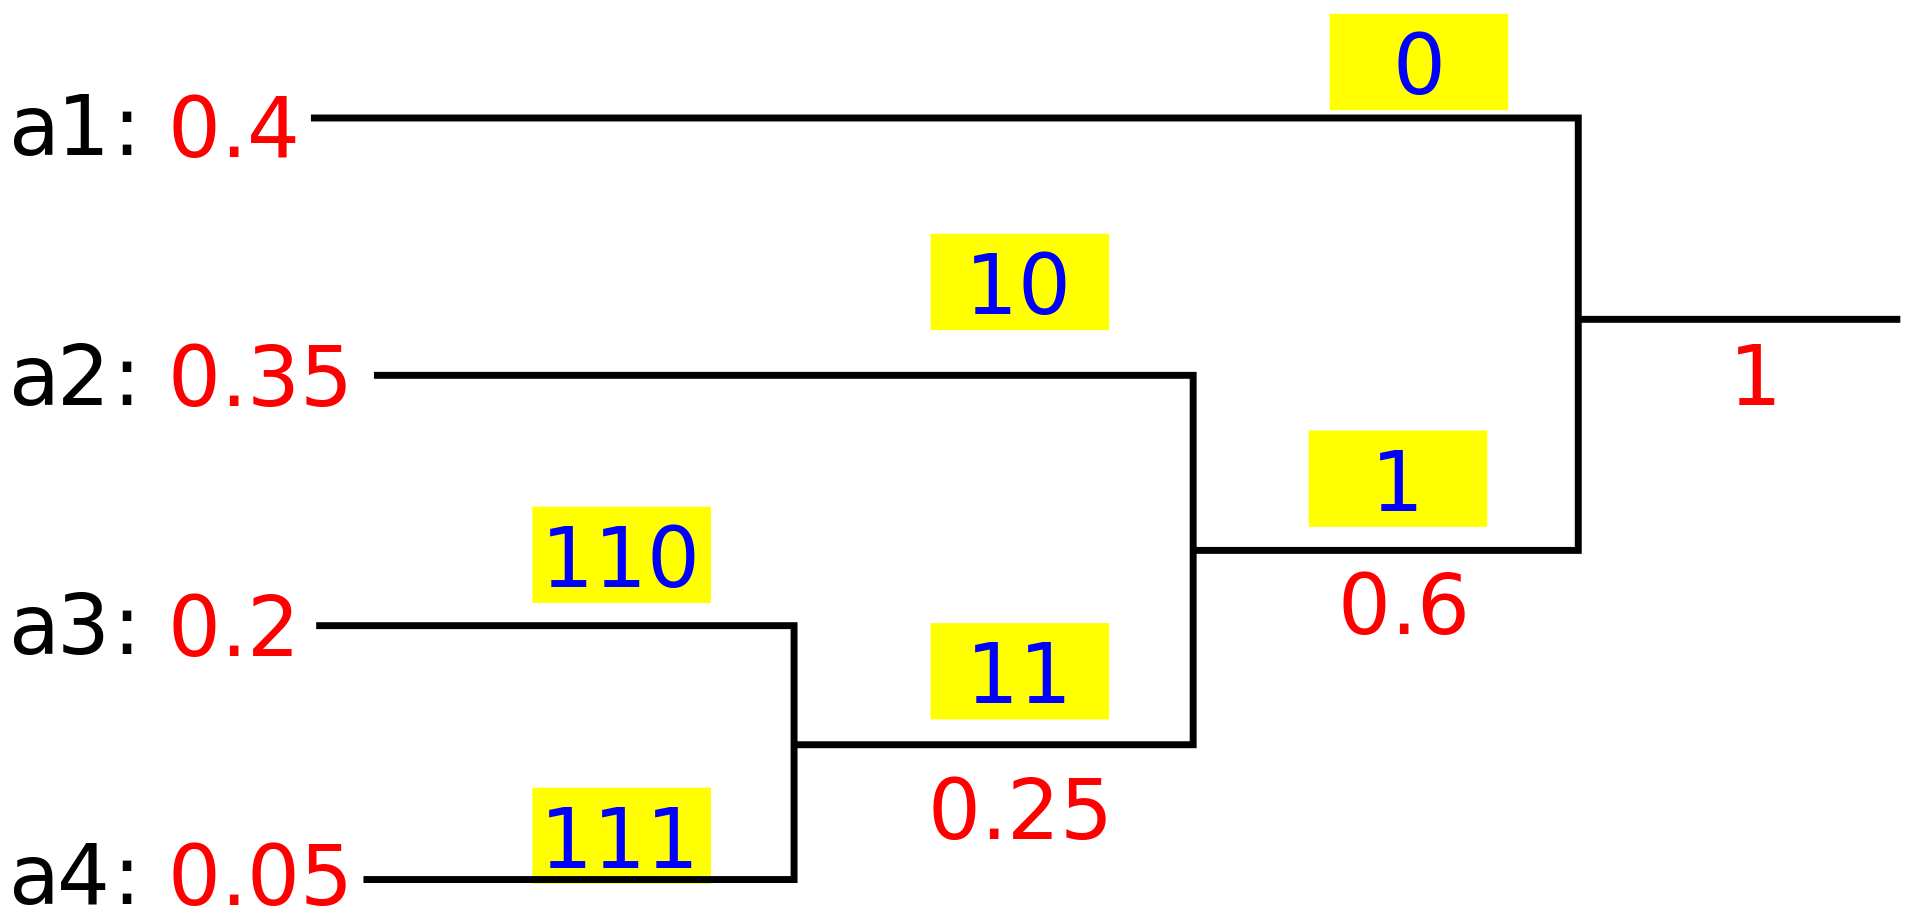
\includegraphics[width=7.5cm]{Huffman_coding_example.png}%
  \caption{\centering Eksempel på Huffmans Tree på data symbolerne a1, a2, a3, a4 \cite{Wiki/Huffman}}\label{Huffmans}%
\end{figure}\\
Figur \ref{Huffmans} er et eksempel på Huffmans tree på data symbolerne {a1, a2, a3, a4}. De røde tal er sandsynligheden for hyppigheden for symbolerne.
Hver route til hver node har et repræsenteret bitværdi (\textit{0} eller \textit{1}). \\
Den repræsenterende kode for symbolerne i Huffmans tree vil blive inddelt ud fra sandsynligheden for hyppigheden for symbolet:
\begin{table}[ht]
  \centering
  \begin{tabular}{ |c|c| }
   \hline
   \textbf{Symbol} & \textbf{Kode} \\
   \hline
   a1 &  0  \\
   \hline
   a2 & 10  \\
   \hline
   a3 &  110 \\
   \hline
   a4 &  111 \\
   \hline
  \end{tabular}
\end{table}
\newpage
\subsection{Eksempel}
Hvis vi tag samme eksempel som brugt i LZ77 algorithmen, ser Huffmans tree således ud:
\begin{figure}[ht]%
  \centering
  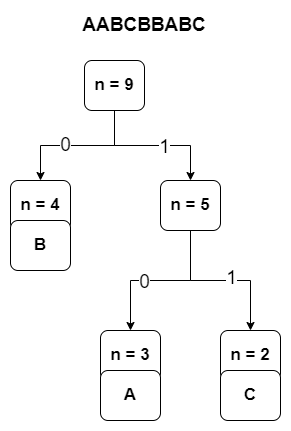
\includegraphics[width=5.5cm]{Huffman_abc_example.png}%
  \caption{\centering \textit{n} er mængden af symbolets hyppighed}%
\end{figure}\\
Den repræsenterende kode for symbolerne i Huffmans tree for eksemplet:
\begin{table}[ht]
  \centering
  \begin{tabular}{ |c|c| }
   \hline
   \textbf{Symbol} & \textbf{Kode} \\
   \hline
   B &  0  \\
   \hline
   A & 10  \\
   \hline
   C &  11 \\
   \hline
  \end{tabular}
\end{table}
\section{Metode og analyse}
Der er adskillige kompressionsalgoritmer og metoder. Den mest kendte algoritme inden for komprimering af filer og billeder er DEFLATE algoritmen. 
DEFLATE algoritmen er en kombination af Huffman coding og LZ77 algoritmerne. Dette opnår fleksibel komprimerings evner som er brugt i forskellige applikationer, 
mest kendt for deres brug i gzip komprimeret filer og PNG-billedfiler.
\subsection{Gennemgang af min kode}
Projektet som jeg har lavet, er en virtuel fremvisning af komprimeringen af billeder. Projektet er en hjemmeside som gør det muligt for brugeren at uploade et billede og få det komprimeret. 
indstillingerne for komprimeringen er både højde, brede og kvalitet af billedet. \\\\
Jeg har med brug af en importeret bibliotek ”Compressorjs”\cite{Compressorjs} som bruger browserens indbygget API canvas.toBlob, til kompensation. 
Dette gør at alle billedfiler som bliver uploadet, er der kun mulighed for en lossy komprimering. Til udvikling af hjemmesiden bruger jeg React og TailwindCSS som framework. \\\\\\
Når brugeren uploader en billedfil til hjemmesiden, bliver filen tildelt kompressionsbiblioteket. Bibliotek komprimerer derefter billedfilen ud fra indstilleringerne som brugeren har valgt:\\
\noindent\begin{minipage}{.4\textwidth}
  \begin{figure}[H]
    \centering
    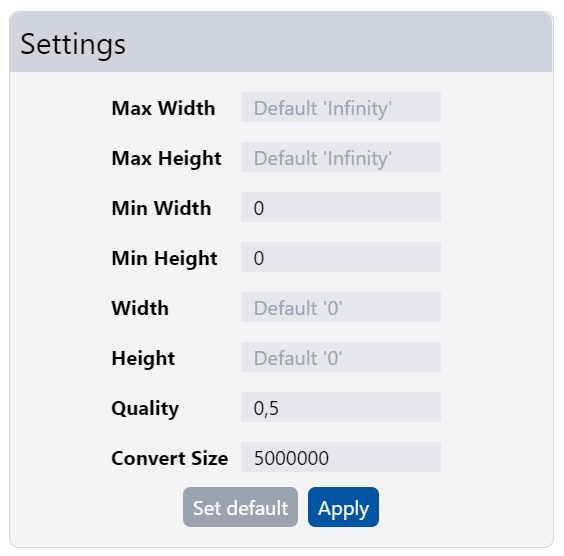
\includegraphics[width=5cm]{2.png}%
    \caption{\centering Illustration af 'Settings'}%
  \end{figure}
  \end{minipage}\hfill
  \begin{minipage}{.55\textwidth}
  \begin{lstlisting}[language=JavaScript, caption=Indsættelse af fil i Compressorjs bibliotek]
if (file.length !== 0) {
  new Compressor(file[0], {
    ...options, // parse user options
    success: (result: File) => {
      // set React hook to result
      setCompressed(result); 
    },
    error(err) {
      // error handeling
      console.log(err.message);
    },
  });
}
  \end{lstlisting}
\end{minipage}\\\\
Det komprimeret billede bliver derefter fremvist til brugeren om både differencen for den komprimeret filstørrelse forhold til det originale billede.
Samt får brugeren mulighed til at downloade det komprimeret billede:\\
\noindent\begin{minipage}{.4\textwidth}
  \begin{figure}[H]
    \centering
    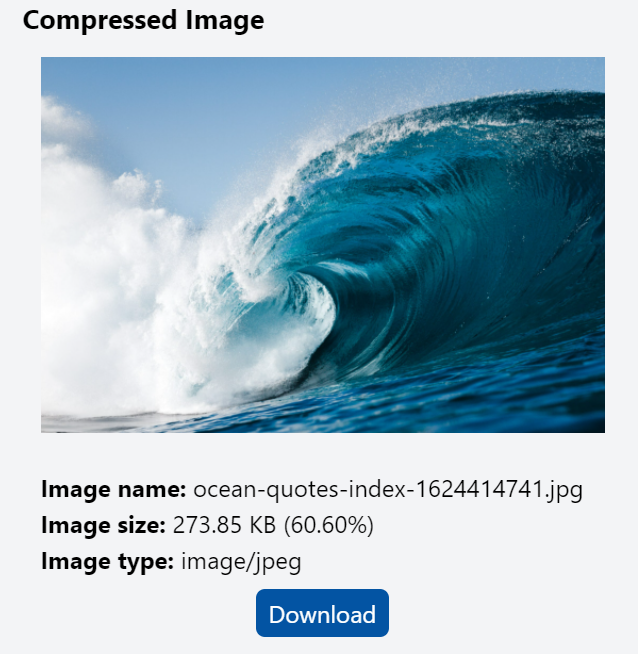
\includegraphics[width=6cm]{1.png}%
    \caption{\centering Illustration af 'preview'}%
  \end{figure}
  \end{minipage}\hfill
  \begin{minipage}{.55\textwidth}
    \begin{lstlisting}[language=JavaScript, caption=Download komprimeret billede med knap]
onClick={() => {
  // get URL from compressed file
  const URL = getImgURL(file); 

  fetch(URL).then((res) => { 
    const a = document.createElement("a");
    a.style.display = "none";
    a.href = res.url;
    a.download = `${name}`; 
    document.body.appendChild(a);
    a.click();
    // Memory cleanup
    window.URL.revokeObjectURL(res.url); 
  });
}}
   \end{lstlisting}
\end{minipage}
Efter en kompression af et billed for \textit{0,1} af kvaliteten af det originale billed, fås en reduktion på 87\% eller 13\% af det originale billed. Dette er en kompression fra $451$ MB til $58$ MB 
\begin{figure}[ht]%
  \centering
  \subfloat[\centering Det originale billed - før kompression]{{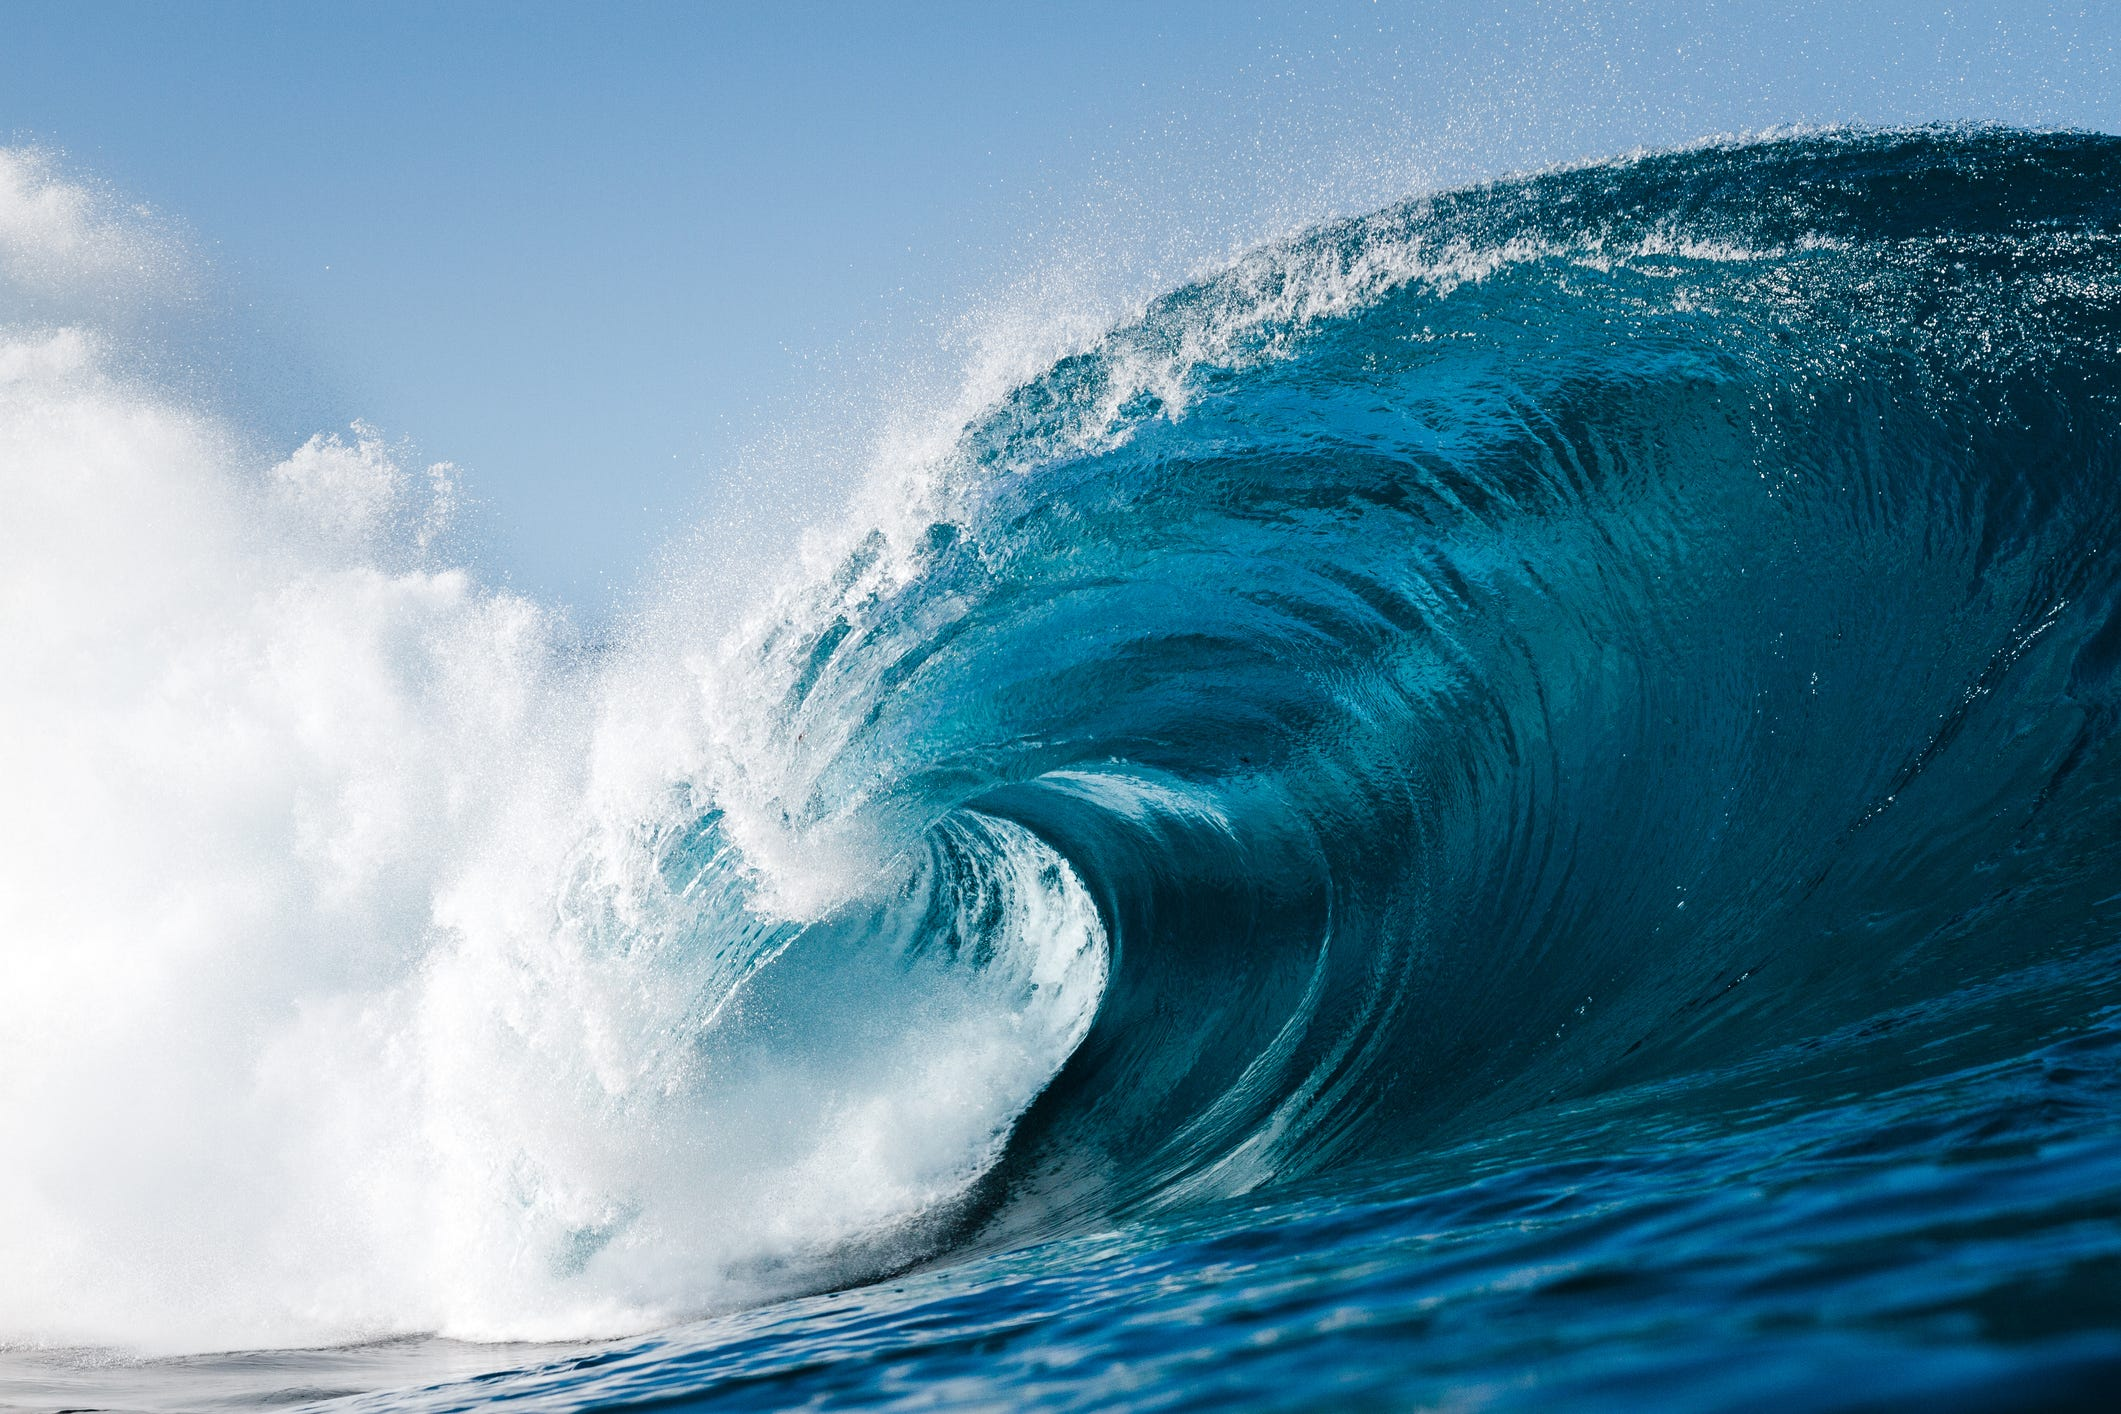
\includegraphics[width=8.25cm]{before.jpg} }}%
  \subfloat[\centering Det komprimere billed - efter kompression]{{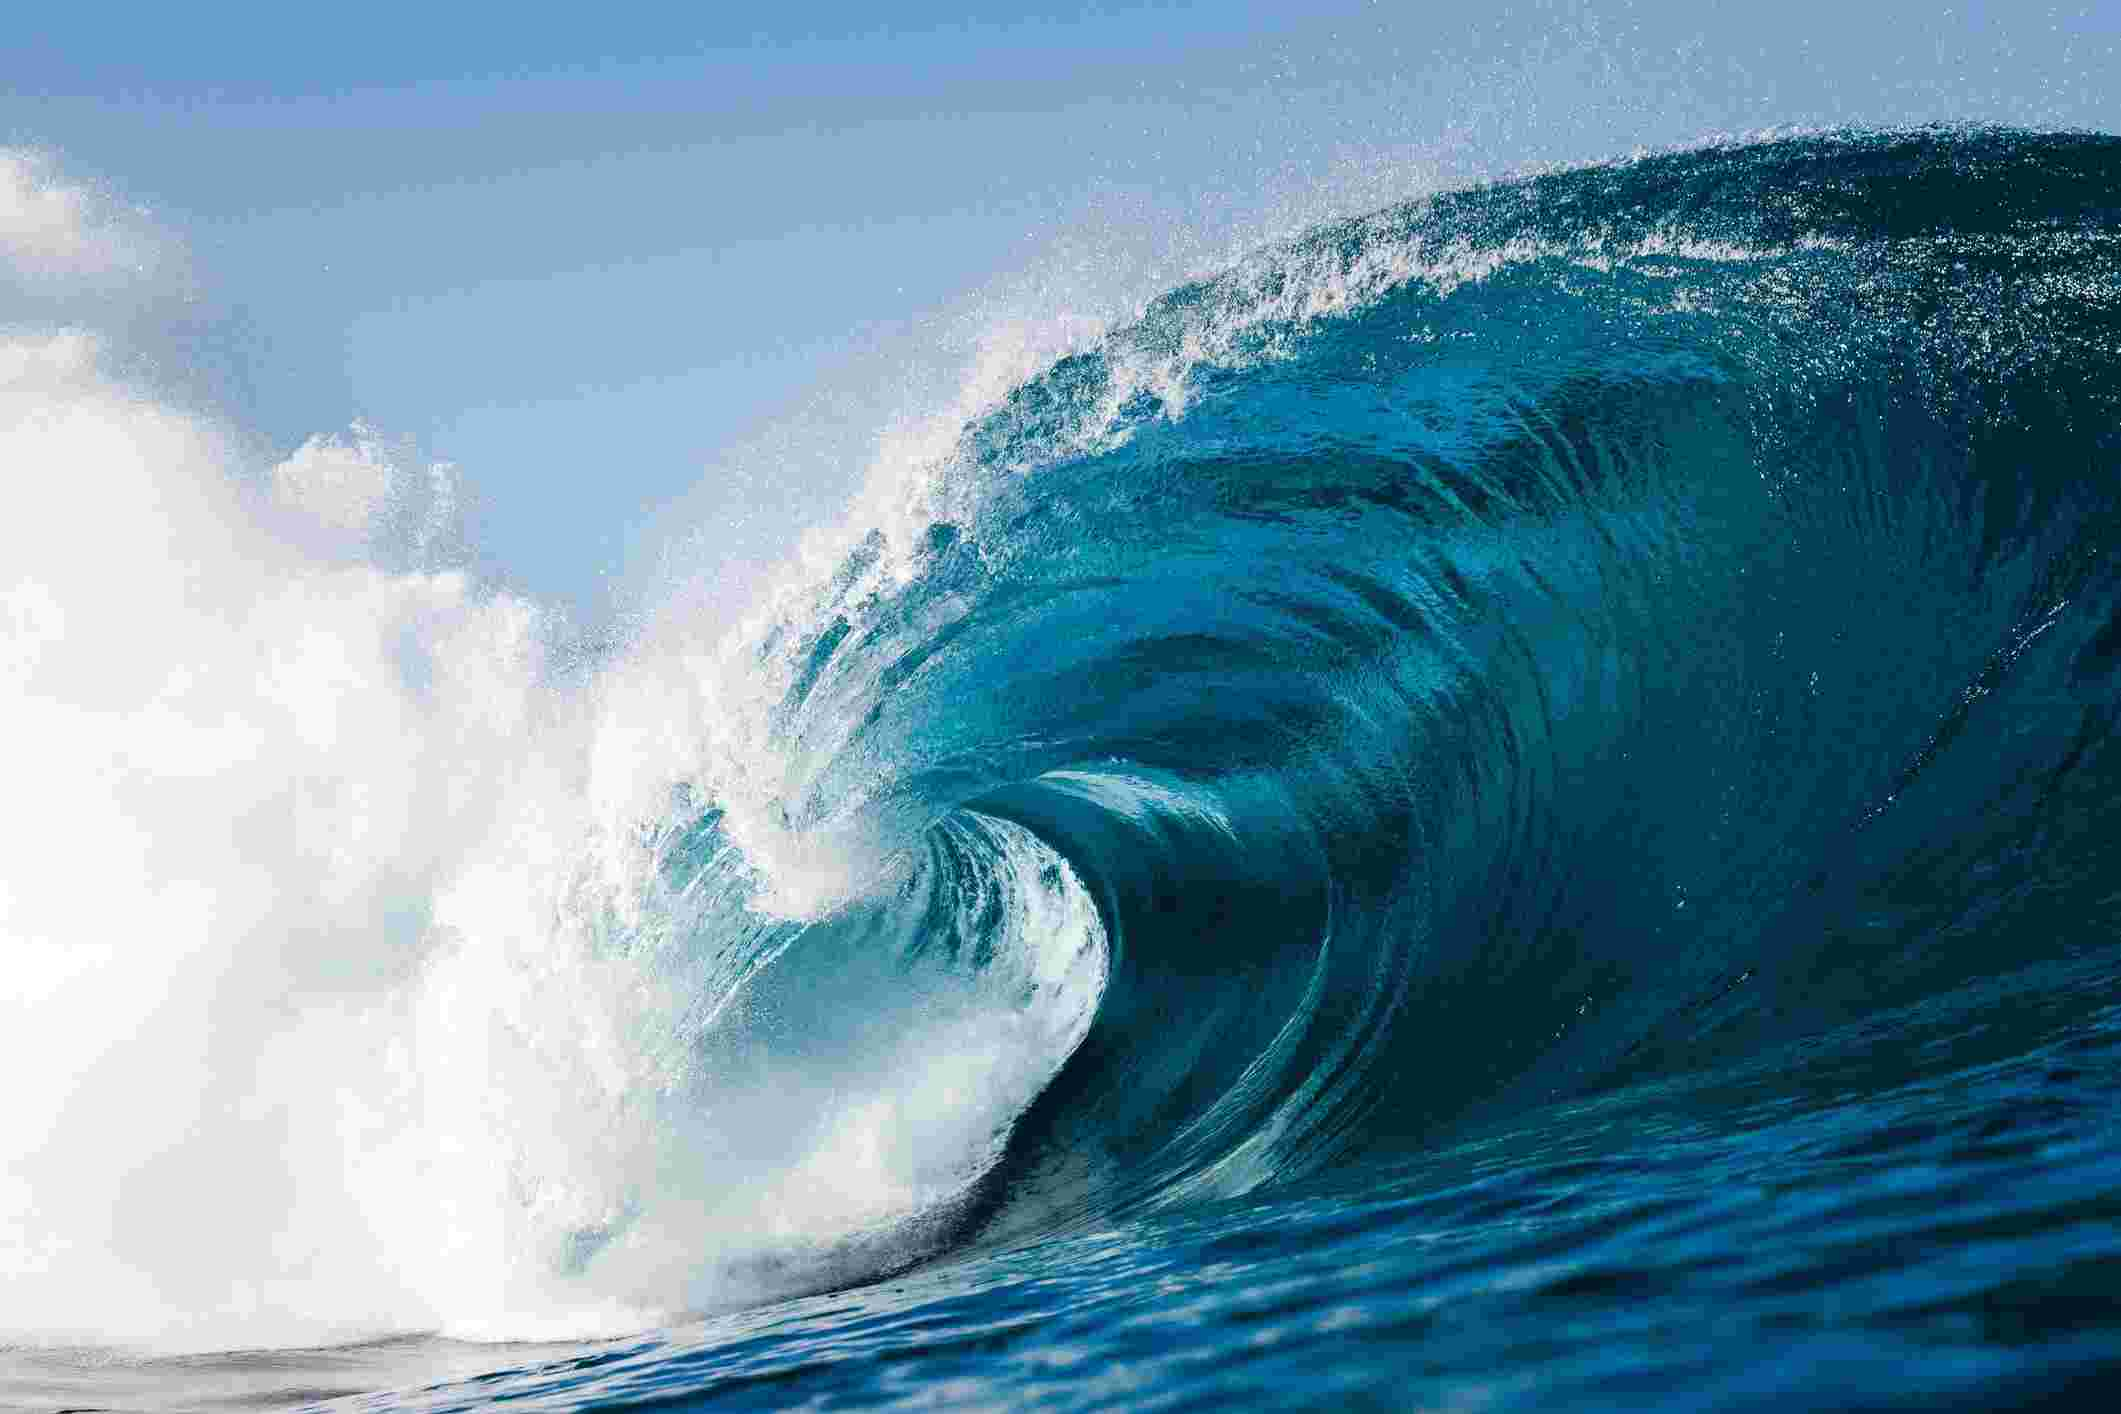
\includegraphics[width=8.25cm]{after.jpg} }}%
\end{figure}
\newpage
\section{Bilag}
\begin{lstlisting}[language=JavaScript, caption=LZ77 Pseudocode]
while input is not empty do
  match := longest repeated occurrence of input that begins in window
  
  if match exists then
      d := distance to start of match
      l := length of match
      c := char following match in input
  else
      d := 0
      l := 0
      c := first char of input
  end if
  
  output (d, l, c)
  
  discard l + 1 chars from front of window
  s := pop l + 1 chars from front of input
  append s to back of window
repeat

\end{lstlisting}
\begin{figure}[ht]%
  \centering
  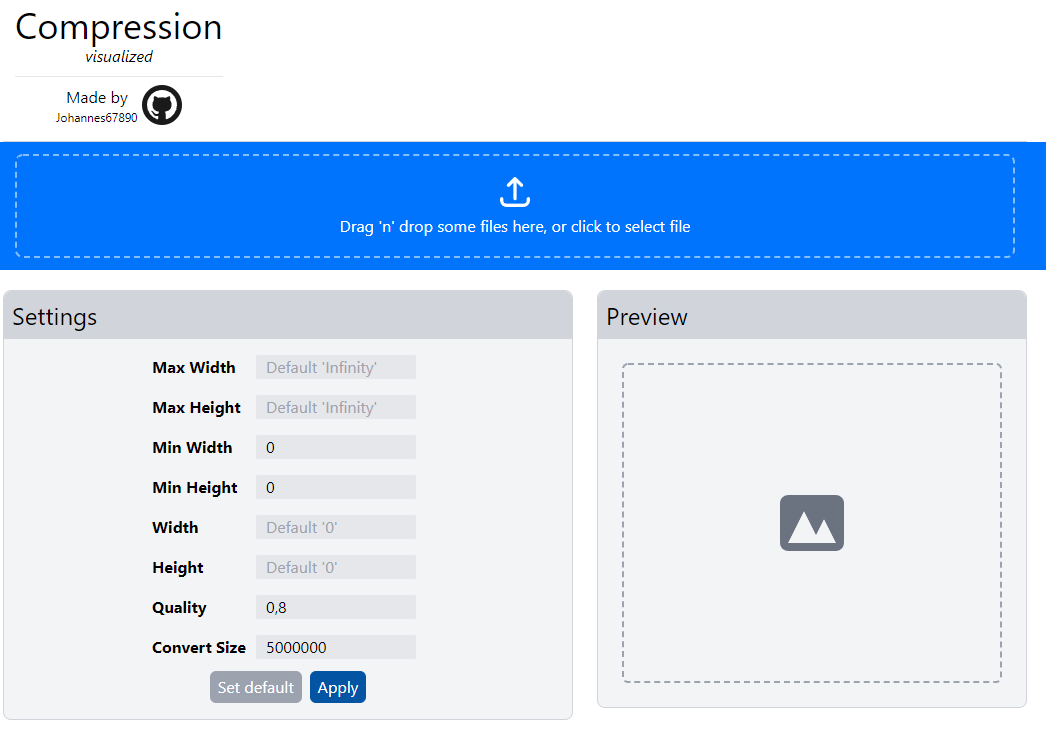
\includegraphics[width=17cm]{Apppreview.png}
  \caption{\centering Illustration af Projekte app}
\end{figure}
\newpage
\printbibliography[title={Litteraturliste}]
\end{document}
